
\section{Introduction}\label{sec_intro}
%[background]
After the pioneering work of \cite{Farrell1957}, \cite{Debreu1951}, and \cite{koopmans1951analysis}, efficiency and productivity analysis have been widely used in empirical studies assessing the performance of decision-making units (DMUs) in terms of converting inputs into outputs. 
Among the parametric and nonparametric frontier models that have been developed in the field of efficiency analysis, Data Envelopment Analysis (DEA) has received plenty of attention for its no needing for prior information of the production function form and capability in multiple output technologies \citep{Fare1985,Fare1994}. 
Efficiency analysis based on DEA is usually assumed that inputs should be shrunk and outputs should be expanded. However, in the real
world, outputs are not always desirable. In the case of undesirable outputs, they should be shrunk to improve efficiency.
In the last decades, with the increasing demand for improving the sustainability of the economic society, scholars and managers gradually recognized that it is vital to consider undesirable output in efficiency and productivity analysis \citep{Chung1997,Mahlberg2011}. Correspondingly, DEA models with the ability to deal with undesirable outputs have been developed and applied in empirical studies, e.g., \citep{Zhou2012,Lin2015}. 

%[introduce existing estimation procedures]
The estimation of nonparametric frontier models can be readily performed in Stata with some user-written commands. 
The {\tt dea} command proposed in \cite{Ji2010} provided a basic tool to estimate radial technical efficiency using the DEA technique in Stata. 
\cite{Badunenko2016} extended {\tt dea} with five new commands that allow users to implement both radial and nonradial technical efficiency estimation, as well as statistical inference in nonparametric frontier models in Stata. 
\cite{Tauchmann2012} introduced two commands, i.e., {\tt orderm} and {\tt orderalpha}, for implementing order-$m$, order-$\alpha$, and free disposal hull efficiency analysis in Stata. 
%[gap]
These commands mentioned above, however, are limited in their capability for performing efficiency and productivity analysis with undesirable outputs. 

%[introduce the command provided here]
Here, we introduce two user-written commands for measuring technical efficiency and productivity change with undesirable outputs in Stata. {\tt teddf} estimates directional distance function (DDF) with undesirable outputs for technical efficiency measurement. Both radial Debreu-Farrell and nonradial Russell measures can be calculated under different assumptions about the production technology, e.g., window, biennial, sequential, and global production technology.
{\tt gtfpch} measures total factor productivity (TFP) change with undesirable outputs using the Malmquist–Luenberger productivity index or the Luenberger indicator. 
%[advantages]
The new commands open up the possibility to do efficiency and productivity analysis with undesirable outputs in Stata in an effortless way, and their results can directly feed to other Stata routines for further analysis. 

%[structure of the present paper]
The remainder of this article unfolds as follows: 
section \ref{sec_method} provides a brief overview of the nonparametric efficiency and productivity change measurement with the consideration of undesirable outputs; 
sections \ref{sec_teddf} and \ref{sec_gtfpch} contain the syntax and explain the options of {\tt teddf} and {\tt gtfpch}, respectively; 
section \ref{sec_example} presents a hypothetical example to show the usage of the two commands; 
and section \ref{sec_conclusion} concludes the article.

\section{The model}\label{sec_method}
%[intro]
In this section, we provide a brief overview of the nonparametric efficiency and productivity measurement with the consideration of undesirable outputs. 
The radial and nonradial directional distance function will be introduced firstly, followed by the description of the measurement of technical efficiency and TFP change using DDFs. 
The exposition here is only introductory. For more details, please refer to the cited works.

\subsection{Directional distance function}
Consider a production unit transforming a vector of nonnegative inputs into a vector of nonnegative desirable outputs and a vector of by-products (undesirable outputs) such as pollution, subject to the constraint imposed by a fixed technology. For the production technology, inputs and desirable outputs are supposed to be strongly disposable. The undesirable outputs are assumed to be weakly disposable, which indicates that the decrease of undesirable outputs is not free but will lead to a deduction in desirable outputs.
If we denote the input, desirable output, and undesirable outputs as $\pmb{x} \in \Re _ + ^N$,  $\pmb{y} \in \Re _ + ^M$, and $\pmb{b} \in \Re _ + ^H$, respectively, the production technology described above can be characterized by the technology set as
\begin{equation}\label{eq_tech}
    T = \{ (\pmb{x},\pmb{y},\pmb{b}) : \pmb{x} \text{ can produce } (\pmb{y},\pmb{b}) \}.
\end{equation}

Then, following \cite{Chung1997}, the radial DDF is defined as
\begin{equation}\label{eq_ddf_r}
    D_r (\pmb{x},\pmb{y},\pmb{b};\pmb{g}) = \sup \{ \beta :((\pmb{x},\pmb{y},\pmb{b}) + \beta \pmb{g}) \in T  \} 
\end{equation}
where $\pmb{g} = (\pmb{g}_x,\pmb{g}_y, \pmb{g}_b) \in \Re _ - ^N \times \Re _ + ^M \times \Re _ - ^H$ is a preassigned nonzero vector, specifying the direction in which the distance between the data point, $(\pmb{x},\pmb{y},\pmb{b})$, and the production frontier is measured. 

Equation \eqref{eq_ddf_r} gives out the most general form of radial DDF. One can define the distance between the DMU and the production frontier in a specific direction by setting different $\pmb{g}$. By way of illustration, we consider the cases of  ${\pmb{g}_1} = (\pmb{0},\pmb{y},\pmb{0})$, ${\pmb{g}_2} = (\pmb{0},\pmb{0},-\pmb{b})$, ${\pmb{g}_3} = (\pmb{0},\pmb{y},-\pmb{b})$, which is widely used in literature. 
Figure \ref{fig_ddf} presents hypothetical one-desirable output (e.g., \textit{GDP}) one-undesirable output (e.g., \textit{CO$_2$}) production processes. 
Conceptually, in Fig. \ref{fig_ddf}, $\overline{\textit{AB}}$ and $\overline{\textit{AC}}$ represent the distance when the direction is ${\pmb{g}_1} = (\pmb{0},\pmb{y},\pmb{0})$ and ${\pmb{g}_2} = (\pmb{0},\pmb{0}, - \pmb{b})$, respectively. The former focuses on economic prosperity, while the latter focuses on environmental protection. Similarly, $\overline{\textit{AD}}$ is the distance when the direction is ${\pmb{g}_3} = (\pmb{0},\pmb{y}, - \pmb{b})$, which describes the maximum increase of desirable output while simultaneously reducing the undesirable output along the direction $(\pmb{y}, - \pmb{b})$. 
Intuitively, the smaller the distance, the closer the DMU is next to the production frontier, and the distance is 0 for the DMU which operates on the production frontier.

\begin{figure}[ht]
    \centering
    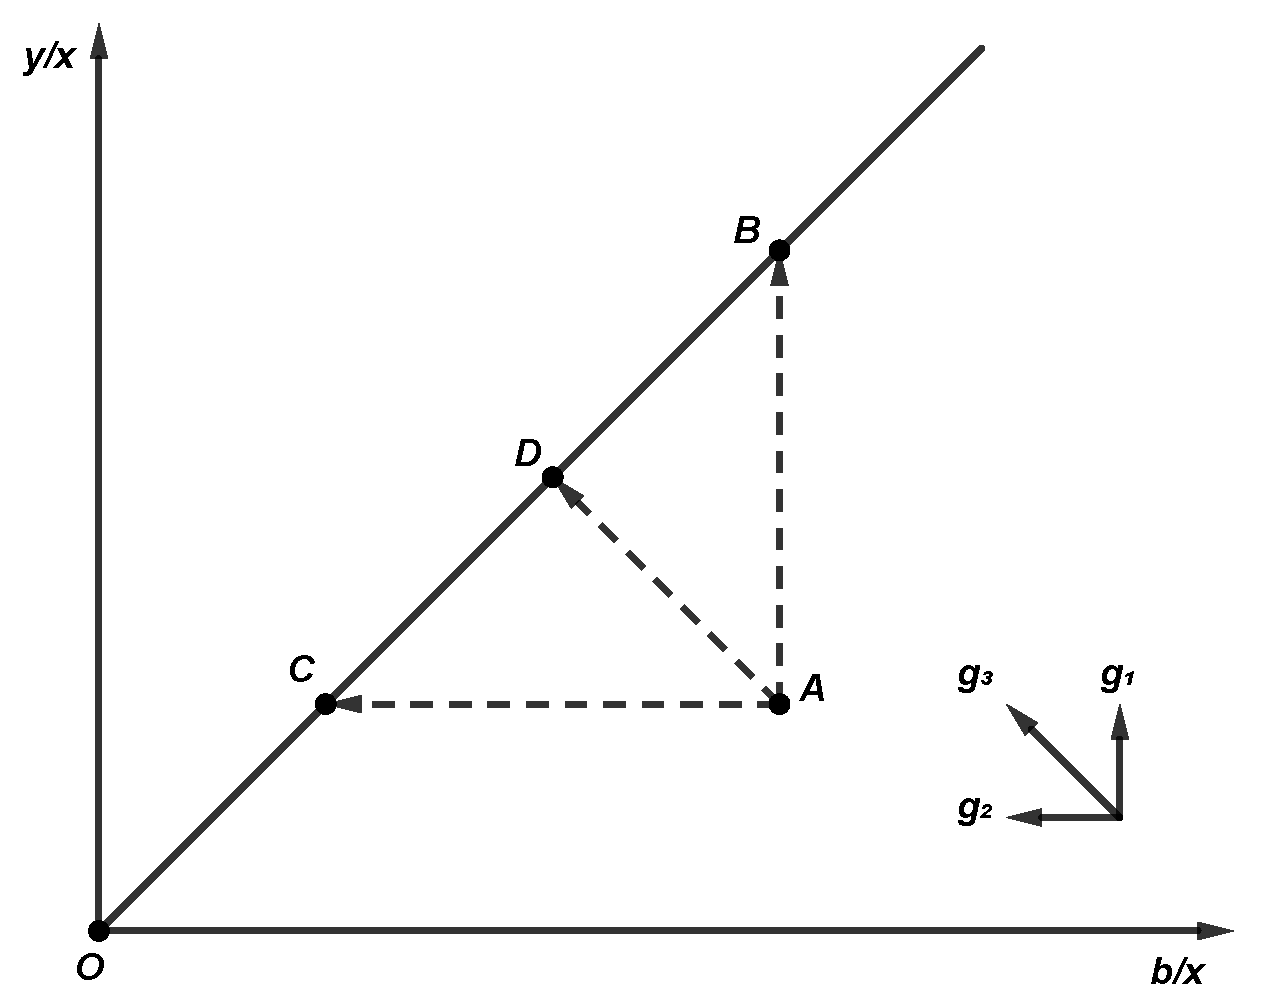
\includegraphics[scale=0.5]{SJF1.pdf}
    \caption{A graphical illustration of directional distance functions} 
    \label{fig_ddf}
\end{figure}

The radial measure expands (shrinks) all outputs or/and inputs proportionally until the production frontier is reached. At the reached frontier point, some but not all outputs (inputs) can be expanded (shrunk) while remaining feasible. If such a possibility is available for a given decision-making unit for some outputs (inputs), then the reference point is said to have slacks in outputs (inputs). Nonradial measures, i.e., the Russell measure, accommodate such slacks \citep{Chambers2002,Fare2010,Zhou2012}.

The nonradial DDF is defined as
\begin{equation}\label{eq_ddf_nr}
    D_{nr} (\pmb{x},\pmb{y},\pmb{b};\pmb{g}) = \sup \{ \pmb{w}^{Transpose} \pmb{\beta} :((\pmb{x},\pmb{y},\pmb{b}) + \textit{diag}(\pmb{\beta}) \cdot \pmb{g}) \in T \} 
\end{equation}
where $\pmb{w}$ denotes a normalized weight vector that is relevant to the numbers of inputs and outputs, and ${\pmb{\beta }} = ({{\pmb{\beta }}_x},{{\pmb{\beta }}_y},{{\pmb{\beta }}_b}) \in {\Re ^N} \times {\Re ^M} \times {\Re ^H}$ denotes the vector of the scaling factors. 
Clearly, the nonradial DDF measure allows the inputs and outputs to be adjusted non-proportionally. Compared with the radial measure in Fig.\ref{fig_ddf}, instead of using a fixed point, e.g., B, C, or D, as the reference point, if the nonradial directional distance function is used, the reference point would be located at any point on the production frontier.
 

\subsection{Measurement of technical efficiency}
To estimate the DDF measure of technical efficiency using the nonparametric technique, the production technology set is derived from observed data. Typically, for the cross-sectional data with $J$ individuals, the production technology set with the assumption of constant return to scale (CRS) is constructed as

\begin{equation}\label{eq_tech_dea}
    T = \left\{ {({\pmb{x}},{\pmb{y}},{\pmb{b}}):\sum\limits_{j = 1}^J {{\lambda _j}{{\pmb{x}}_j} \le {\pmb{x}},\sum\limits_{j = 1}^J {{\lambda _j}{{\pmb{y}}_j} \ge {\pmb{y}},} \sum\limits_{j = 1}^J {{\lambda _j}{{\pmb{b}}_j} = {\pmb{b}},} }  {\pmb{\lambda }} \ge 0} \right\}.
\end{equation}

For variable returns to scale (VRS), $\sum_{j=1}^{J} \lambda_j =1$ is added to the above equation. That is,
\begin{equation}\label{eq_tech_dea_v}
    T = \left\{ {({\pmb{x}},{\pmb{y}},{\pmb{b}}):\sum\limits_{j = 1}^J {{\lambda _j}{{\pmb{x}}_j} \le {\pmb{x}},\sum\limits_{j = 1}^J {{\lambda _j}{{\pmb{y}}_j} \ge {\pmb{y}},} \sum\limits_{j = 1}^J {{\lambda _j}{{\pmb{b}}_j} = {\pmb{b}},} }  {\pmb{\lambda }} \ge 0}, \sum\limits_{j = 1}^J {{\lambda _j} = 1} \right\}.
\end{equation}

In the panel data context, the time-series dimension can provide more information on the production technology. Researchers have proposed different types of production technology sets such as global, sequential, window, biennial, and contemporaneous production technology. The production technology set at the time $t$ as follows:

\begin{equation}\label{eq_tech_dea_panel}
	T(t) = \left\{ {({\pmb{x}},{\pmb{y}},{\pmb{b}}):\sum\limits_{\tau \in \Gamma_t }\sum\limits_{j = 1}^J {{\lambda _{j\tau}}{{\pmb{x}}_{j\tau}} \le {\pmb{x}},\sum\limits_{\tau \in \Gamma_t }\sum\limits_{j = 1}^J {{\lambda _{j\tau}}{{\pmb{y}}_{j\tau}} \ge {\pmb{y}},} \sum\limits_{\tau \in \Gamma_t }\sum\limits_{j = 1}^J {{\lambda _{j\tau}}{{\pmb{b}}_{j\tau}} = {\pmb{b}},} } {\pmb{\lambda }} \ge 0} \right\}.
\end{equation}


The time range, $\tau \in \Gamma_t$, for different types of production technology set are shown in Fig.\ref{fig_time}. In the global production technology, $\tau \in \Gamma_t$ is expressed as $\tau \leq t_{max}$, where $t_{max}$ is the last period in the sample. In the sequential production technology, $\tau \in \Gamma_t$ is expressed as $\tau \leq t$. In the window production technology, $\tau \in \Gamma_t$ is expressed as $t - h \leq \tau \leq t + h $, where $h$ is the bandwidth.  In the biennial production technology, $\tau \in \Gamma_t$ is expressed as $t \leq \tau \leq t + 1 $. In the contemporaneous production technology, $\tau \in \Gamma_t$ is expressed as $\tau=t$. 

\begin{figure}[ht]
    \centering
    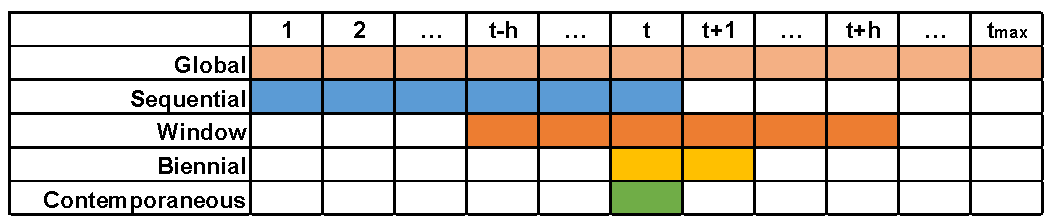
\includegraphics[scale=0.65]{SJF2.pdf}
    \caption{Timing assumption of different type of production technology sets} 
    \label{fig_time}
\end{figure}


Then, the radial DDF measure of inefficiency under the CRS assumption can be estimated by solving the following linear programming problem,
\begin{equation}\begin{split}\label{eq_eff_r}
    D_r (\pmb{x},\pmb{y},\pmb{b};\pmb{g}) 
    = &\max _{\beta,\pmb{\lambda}} \beta  \\ 
    \text{s.t.} &\sum\limits_{j = 1}^J {\lambda _j \pmb{x}_j \le \pmb{x} + \beta \pmb{g}_x}, \\ 
                &\sum\limits_{j = 1}^J {\lambda _j \pmb{y}_j \ge \pmb{y} + \beta \pmb{g}_y}, \\ 
                &\sum\limits_{j = 1}^J {\lambda _j \pmb{b}_j = \pmb{b} + \beta \pmb{g}_b}, \\ 
                &\lambda _j \ge 0, j = 1,...,J.
\end{split}\end{equation}
This technology set is based on the assumption of constant return to scale. For VRS assumption, $\sum_{j=1}^{J} \lambda_j =1$ is added to above constraints.

In Eq.(7), the left-hand side of the constraints construct the production frontier using the convex hull of the observation data and the right-hand side allows the assessed DMU to adjust the inputs ($x$), the desirable outputs ($y$) and undesirable outputs ($b$) alongside the direction of $(g_x,g_y,g_b)$. The directional distance function seeks to maximize the reduction of inputs and undesirable outputs and the expansion of the desirable output in means of $(x+\beta g_x, y+ \beta g_y, b+\beta g_b)$ given the production technology. 

Similarly, the nonradial DDF measure of inefficiency considering the undesirable outputs can be obtained by solving the following linear programming problem.
\begin{equation}\begin{split}\label{eq_eff_nr}
    D_{nr} (\pmb{x},\pmb{y},\pmb{b};\pmb{g}) 
    = &\max _{\pmb{\beta},\pmb{\lambda}} \pmb{w}^{T} \pmb{\beta}  \\ 
    \text{s.t.} &\sum\limits_{j = 1}^J {\lambda _j \pmb{x}_j \le \pmb{x} + diag(\pmb{\beta}_x)\cdot \pmb{g}_x}, \\ 
                &\sum\limits_{j = 1}^J {\lambda _j \pmb{y}_j \ge \pmb{y} + diag(\pmb{\beta}_y)\cdot \pmb{g}_y}, \\ 
                &\sum\limits_{j = 1}^J {\lambda _j \pmb{b}_j = \pmb{b} + diag(\pmb{\beta}_b)\cdot \pmb{g}_b}, \\ 
                &\pmb{\beta} \ge 0; \lambda _j \ge 0, j = 1,...,J.
\end{split}\end{equation}
For variable returns to scale assumption, $\sum_{j=1}^{J} \lambda_j =1$ is added to above constraints. 

Unlike the directional distance function shown in Eq.(7), the nonradial directional distance function allows each component of inputs, desirable outputs, and undesirable outputs to adjust in varying proportions. The nonradial DDF is the maximum weighted sum of the adjustment components ($\beta$) such that $(diag(\beta_x)\cdot g_x,diag(\beta_y)\cdot g_y,diag(\beta_b)\cdot g_b)$ can be produced given the production technology. 


For the panel data case, the radial DDF measure of inefficiency under the CRS assumption can be estimated by solving the following linear programming problem,
\begin{equation}\begin{split}\label{eq_eff_r_panel}
    D_r (\pmb{x},\pmb{y},\pmb{b};\pmb{g}) 
    = &\max _{\beta,\pmb{\lambda}} \beta  \\ 
    \text{s.t.} &\sum\limits_{\tau \in \Gamma_t }\sum\limits_{j = 1}^J {{\lambda _{j\tau}}{{\pmb{x}}_{j\tau}} \le \pmb{x} + \beta \pmb{g}_x}, \\ 
                &\sum\limits_{\tau \in \Gamma_t }\sum\limits_{j = 1}^J {{\lambda _{j\tau}}{{\pmb{y}}_{j\tau}} \ge \pmb{y} + \beta \pmb{g}_y}, \\ 
                &\sum\limits_{\tau \in \Gamma_t }\sum\limits_{j = 1}^J {{\lambda _{j\tau}}{{\pmb{b}}_{j\tau}} = \pmb{b} + \beta \pmb{g}_b}, \\ 
                &\lambda _{j\tau} \ge 0, j = 1,...,J.
\end{split}\end{equation}

Similarly, for the panel data case, the nonradial DDF measure of inefficiency can be estimated by solving the following linear programming problem,
\begin{equation}\begin{split}\label{eq_eff_nr_panel}
    D_{nr} (\pmb{x},\pmb{y},\pmb{b};\pmb{g}) 
    = &\max _{\pmb{\beta},\pmb{\lambda}} \pmb{w}^{T} \pmb{\beta}  \\ 
    \text{s.t.} &\sum\limits_{\tau \in \Gamma_t }\sum\limits_{j = 1}^J {{\lambda _{j\tau}}{{\pmb{x}}_{j\tau}} \le \pmb{x} + diag(\pmb{\beta}_x)\cdot \pmb{g}_x}, \\ 
                &\sum\limits_{\tau \in \Gamma_t }\sum\limits_{j = 1}^J {{\lambda _{j\tau}}{{\pmb{y}}_{j\tau}} \ge \pmb{y} + diag(\pmb{\beta}_y)\cdot \pmb{g}_y}, \\ 
                &\sum\limits_{\tau \in \Gamma_t }\sum\limits_{j = 1}^J {{\lambda _{j\tau}}{{\pmb{b}}_{j\tau}} = \pmb{b} + diag(\pmb{\beta}_b)\cdot \pmb{g}_b}, \\ 
                &\pmb{\beta} \ge 0; \lambda_{j\tau} \ge 0, j = 1,...,J.
\end{split}\end{equation}


\subsection{Measurement of total factor productivity change}
The measurement of productivity change has traditionally focused on measuring marketable (desirable) outputs of DMUs relative to paid factors of production. 
This approach, which typically ignores the production of by-products such as pollution, can yield biased measures of productivity growth \citep{Chung1997}. 
For example, firms in industries that face environmental regulations would typically find that their productivity is adversely affected since the costs of abatement capital would typically be included on the input side, but no account would be made of the reduction in pollutants on the output side.

\cite{Chung1997} has introduced a productivity index based on the radial DDF measure, called the Malmquist-Luenberger productivity index, which credits the reduction of undesirable outputs, e.g., pollution, while simultaneously crediting increases in desirable outputs. Considering two adjacent periods, denoted as $s$ and $t$. respectively. If we choose the direction to be ${\pmb{g}} = (\pmb{0},\pmb{y}, - \pmb{b})$, the output-oriented Malmquist-Luenberger productivity index with undesirable outputs is defined as
\begin{equation}\label{eq_mpi}
    \textit{ML} %_{\pmb{g}} ({{\pmb{x}}^s},{{\pmb{y}}^s},{{\pmb{b}}^s},{{\pmb{x}}^t},{{\pmb{y}}^t},{{\pmb{b}}^t}) 
    = {\left[ {
    \frac{{1 + D _r^t({{\pmb{x}}^s},{{\pmb{y}}^s},{{\pmb{b}}^s};{\pmb{g}})}}{{1 + D _r^t({{\pmb{x}}^t},{{\pmb{y}}^t},{{\pmb{b}}^t};{\pmb{g}})}} \times \frac{{1 + D _r^s({{\pmb{x}}^s},{{\pmb{y}}^s},{{\pmb{b}}^s};{\pmb{g}})}}{{1 + D _r^s({{\pmb{x}}^t},{{\pmb{y}}^t},{{\pmb{b}}^t};{\pmb{g}})}}  } \right]^{1/2}}.
\end{equation}
To avoid an arbitrary choice between base years, an geometric mean of a fraction-based Malmquist-Luenberger productivity index in base year $t$ (first fraction) and $s$ (second fraction) has been taken. The Malmquist–Luenberger measure indicates productivity improvements if their values are greater than one and decreases in productivity if the values are less than one. 

The Malmquist-Luenberger productivity index can be decomposed into two components \citep{Chung1997}, one accounting for efficiency change (\textit{MLEFFCH}), and one measuring technology change (\textit{MLTECH}):
\begin{equation}
    \textit{MLEFFCH} %_{\pmb{g}} ({{\pmb{x}}^s},{{\pmb{y}}^s},{{\pmb{b}}^s},{{\pmb{x}}^t},{{\pmb{y}}^t},{{\pmb{b}}^t}) 
    = \frac{{1 + D _r^s({{\pmb{x}}^s},{{\pmb{y}}^s},{{\pmb{b}}^s};{\pmb{g}})}}{{1 + D _r^t({{\pmb{x}}^t},{{\pmb{y}}^t},{{\pmb{b}}^t};{\pmb{g}})}}
\end{equation}
and,
\begin{equation}
    \textit{MLTECH} %_{\pmb{g}} ({{\pmb{x}}^s},{{\pmb{y}}^s},{{\pmb{b}}^s},{{\pmb{x}}^t},{{\pmb{y}}^t},{{\pmb{b}}^t}) 
    = {\left[ {\frac{{1 + D _r^t({{\pmb{x}}^s},{{\pmb{y}}^s},{{\pmb{b}}^s};{\pmb{g}})}}{{1 + D _r^s({{\pmb{x}}^s},{{\pmb{y}}^s},{{\pmb{b}}^s};{\pmb{g}})}} 
    \times 
    \frac{{1 + D _r^t({{\pmb{x}}^t},{{\pmb{y}}^t},{{\pmb{b}}^t};{\pmb{g}})}}{{1 + D _r^s({{\pmb{x}}^t},{{\pmb{y}}^t},{{\pmb{b}}^t};{\pmb{g}})}}} \right]^{1/2}}.
\end{equation}

Based on the pioneering work in \cite{Chambers2002}, another productivity measure called the Luenberger productivity indicator is also widely used to account for productivity change. 
The Luenberger productivity indicator based on radial DDF measures is defined as
\begin{equation}\begin{split}\label{eq_li_r}
    \textit{L} %({{\pmb{x}}^s},{{\pmb{y}}^s},{{\pmb{b}}^s},{{\pmb{x}}^t},{{\pmb{y}}^t},{{\pmb{b}}^t}) 
    = & \left[ (D _r^t({{\pmb{x}}^s},{{\pmb{y}}^s},{{\pmb{b}}^s};{\pmb{g}}) - D _r^t({{\pmb{x}}^t},{{\pmb{y}}^t},{{\pmb{b}}^t};{\pmb{g}}) \right] \times \frac{1}{2} \\ 
    + & \left[ D _r^s({{\pmb{x}}^s},{{\pmb{y}}^s},{{\pmb{b}}^s};{\pmb{g}}) - D _r^s({{\pmb{x}}^t},{{\pmb{y}}^t},{{\pmb{b}}^t};{\pmb{g}})) \right] \times \frac{1}{2}.
\end{split}\end{equation}
Again, to avoid an arbitrary choice between base years, an arithmetic mean of a difference based Luenberger productivity index in base year $t$ (first difference) and $s$ (second difference) has been taken. 
Productivity improvements are indicated by positive values and declines by negative values. 

In the spirit of decomposition of Malmquist–Luenberger productivity index, the Luenberger productivity indicator based on radial DDFs can also be decomposed into two component measures, i.e., an efficiency change component \citep{Mahlberg2011},
\begin{equation}
    \textit{LEFFCH} %({{\pmb{x}}^s},{{\pmb{y}}^s},{{\pmb{b}}^s},{{\pmb{x}}^t},{{\pmb{y}}^t},{{\pmb{b}}^t}) 
    = D _r^s({{\pmb{x}}^s},{{\pmb{y}}^s},{{\pmb{b}}^s};{\pmb{g}}) - D _r^t({{\pmb{x}}^t},{{\pmb{y}}^t},{{\pmb{b}}^t};{\pmb{g}})
\end{equation}
and a technical change component,
\begin{equation}\begin{split}
    \textit{LTECH} %({{\pmb{x}}^s},{{\pmb{y}}^s},{{\pmb{b}}^s},{{\pmb{x}}^t},{{\pmb{y}}^t},{{\pmb{b}}^t}) 
    = & \left[ D _r^t({{\pmb{x}}^t},{{\pmb{y}}^t},{{\pmb{b}}^t};{\pmb{g}}) - D _r^s({{\pmb{x}}^t},{{\pmb{y}}^t},{{\pmb{b}}^t};{\pmb{g}}) \right] \times \frac{1}{2} \\ 
    + & \left[ (D _r^t({{\pmb{x}}^s},{{\pmb{y}}^s},{{\pmb{b}}^s};{\pmb{g}}) - D _r^s({{\pmb{x}}^s},{{\pmb{y}}^s},{{\pmb{b}}^s};{\pmb{g}}) \right] \times \frac{1}{2}.
\end{split}\end{equation}
The Luenberger indicator based on radial DDFs is expressed as the sum of \textit{LEFFCH} and \textit{LTECH}. \textit{LEFFCH} captures the average gain/loss due to the difference in technical efficiency from period $s$ to period $t$. \textit{LTECH} captures the average gain/loss due to the shift in technology from period $s$ to period $t$.

Like any radial measure of efficiency estimated using DEA technologies, DDF overestimates the efficiency of a firm when there are non-zero slacks that remain in the constraints after the full radial efficiency is achieved. 
To account for these slacks, \cite{Fare2010} proposed a slacks-based measure of efficiency based on nonradial directional distance function. Another type of Luenberger indicator, called the non-proportional Luenberger indicator, can be constructed based on the nonradial DDFs \citep{Mahlberg2011}. 

The Luenberger productivity indicator based on nonradial DDFs is defined as
\begin{equation}\begin{split}\label{eq_li_nr}
    \textit{L} %({{\pmb{x}}^s},{{\pmb{y}}^s},{{\pmb{b}}^s},{{\pmb{x}}^t},{{\pmb{y}}^t},{{\pmb{b}}^t}) 
    = & \left[ (D _{nr}^t({{\pmb{x}}^s},{{\pmb{y}}^s},{{\pmb{b}}^s};{\pmb{g}}) - D _{nr}^t({{\pmb{x}}^t},{{\pmb{y}}^t},{{\pmb{b}}^t};{\pmb{g}}) \right] \times \frac{1}{2} \\ 
    + & \left[ D _{nr}^s({{\pmb{x}}^s},{{\pmb{y}}^s},{{\pmb{b}}^s};{\pmb{g}}) - D _{nr}^s({{\pmb{x}}^t},{{\pmb{y}}^t},{{\pmb{b}}^t};{\pmb{g}})) \right] \times \frac{1}{2}.
\end{split}\end{equation}

The non-proportional Luenberger productivity indicator can also be decomposed into two parts \citep{Mahlberg2011}. An efficiency change component,
\begin{equation}
    \textit{LEFFCH} %({{\pmb{x}}^s},{{\pmb{y}}^s},{{\pmb{b}}^s},{{\pmb{x}}^t},{{\pmb{y}}^t},{{\pmb{b}}^t}) 
    = D _{nr}^s({{\pmb{x}}^s},{{\pmb{y}}^s},{{\pmb{b}}^s};{\pmb{g}}) - D _{nr}^t({{\pmb{x}}^t},{{\pmb{y}}^t},{{\pmb{b}}^t};{\pmb{g}})
\end{equation}
and a technical change component,
\begin{equation}\begin{split}
    \textit{LTECH} %({{\pmb{x}}^s},{{\pmb{y}}^s},{{\pmb{b}}^s},{{\pmb{x}}^t},{{\pmb{y}}^t},{{\pmb{b}}^t}) 
    = & \left[ D _{nr}^t({{\pmb{x}}^t},{{\pmb{y}}^t},{{\pmb{b}}^t};{\pmb{g}}) - D _{nr}^s({{\pmb{x}}^t},{{\pmb{y}}^t},{{\pmb{b}}^t};{\pmb{g}}) \right] \times \frac{1}{2} \\ 
    + & \left[ (D _{nr}^t({{\pmb{x}}^s},{{\pmb{y}}^s},{{\pmb{b}}^s};{\pmb{g}}) - D _{nr}^s({{\pmb{x}}^s},{{\pmb{y}}^s},{{\pmb{b}}^s};{\pmb{g}}) \right] \times \frac{1}{2}.
\end{split}\end{equation}


\subsection{Statistical inference for technical efficiency and productivity index}

Efficiency and productivity analysis are widely applied in benchmarking(relative performance evaluations). The models introduced above are based on the DEA methods which are typically considered to be deterministic. Specifically, the efficiency/productivity is measured relative to the estimated production frontiers constructed by sample observations. Consequently, the measures of efficiency/productivity might be sensitive to the sampling variations. In view of this, researchers have devoted themselves to exploring the statistical properties of the DEA-type estimators. For instance, \cite{banker1993} and \cite{Kneip1998} established consistency and convergence rates of DEA efficiency estimators. \cite{kneip2008} derived the asymptotic distribution of Farrell measure of technical efficiency (one of the radial DEA estimators) in cases with multiple inputs and outputs. Generally speaking, many DEA-type efficiency estimators have been proposed. But few have been known on their asymptotic distribution. 

To implement statistical inference for DEA-type efficiency estimators, \cite{Simar1998} proposed a smoothed bootstrapping procedure. But the consistency of the smooth bootstrapping method has not been proved. Based on the asymptotic theorems developed in \cite{kneip2008}, they presented another two consistent bootstrapping procedures for Farrell measure of technical efficiency: the subsampling approach and the double-smooth bootstrap. \cite{simar2012} showed that the directional distance function estimators shared the known properties of the traditional radial DEA estimators and adapted the subsampling approach and the double-smooth bootstrap to this context. In the context of nonradial DEA estimators, \cite{Badunenko2020} proposed a bootstrap method for Russell measures of technical efficiency. \cite{Badunenko2016} incorporated the bootstrap procedures in their Stata commands {\tt teradialbc} and {\tt tenonradialbc}. It is worth pointing out that the bootstrap methods mentioned above mainly focus on the cross-sectional data. In the panel data cases, there are some difficulties in applying the smooth/double-smooth bootstrapping methods. Because considering the possibility of temporal correlation, they require nonparametric estimation of a high dimensional density which might suffer from the curse of dimensionality. On the contrary, the subsampling approach can be easily adapted to accommodate the panel data structure by subsampling with clusters. Thus, we incorporate the subsampling approach in our Stata command ({\tt teddf}) for statistical inference.

Regarding the statistical inference for DEA-based productivity indexes, \cite{simar2019} established the asymptotic theorems for nonparametric Malmquist indices. \cite{simar1999}  proposed a bootstrap estimation procedure for obtaining confidence intervals for Malmquist indices of productivity and their decompositions. But until now, the statistical properties of the Malmquist-Luenberger productivity index and the Luenberger productivity indicator are still unknown. Intuitively, the subsampling approach can be adapted to these contexts with the knowledge of the convergence rates. Nevertheless, it is still an open issue. 


\endinput
